
	 % \hfill
	 \begin{figure}[!b]
	 	\centering 
	 	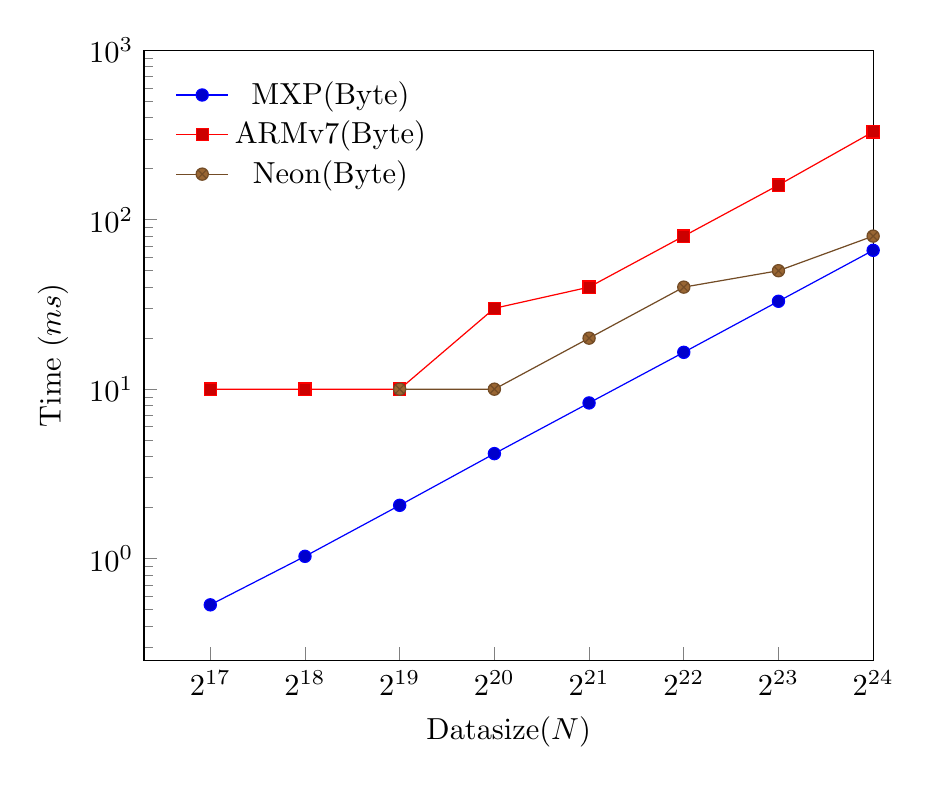
\begin{tikzpicture}[scale = 1.1]
	 	\begin{semilogyaxis}[
	 	xlabel=Datasize$(N)$,
	 	ylabel=Time $(ms)$,
	 	% 	scaled ticks=base 10:-5,
	 	xtick pos=left,
	 	ytick pos=left,
	 	ymax = 1000,
	 	xmax = 16777216,
	 	%	 ymode=log,log ticks with fixed point,
	 	%	grid=major,
	 	%   symbolic y coords={0.4239, 0.847, 1.67, 3.33, 6.69, 13.33,26.63,54.41},
	 	%   ytick={data},
	 	symbolic x coords={131072,262144,524288,1048576,2097152,4194304,8388608,16777216},
	 	xtick=data,
	 	xticklabels={$2^{17}$,$2^{18}$,$2^{19}$,$2^{20}$,$2^{21}$,$2^{22}$,$2^{23}$,$2^{24}$},
	 	%	symbolic y coords={0.4239,0.847,1.67,3.33,6.69,13.33,26.63,54.41,70,150,290,560},
	 	width = 10cm,
	 	xmode = normal,
	 	legend pos=north west,
	 	legend style={draw=none}
	 	]    
	 	
	   	\addplot plot coordinates {
	   		(131072,     0.534)
	   		(262144,     1.032)
	   		(524288,    2.064)
	   		(1048576,    4.166)
	   		(2097152,    8.294)
	   		(4194304,    16.50)
	   		(8388608,   33.01)
	   		(16777216,  65.97)
	   		
	   	};
%	   	\addplot plot coordinates {
%	   		(131072,     0.71)
%	   		(262144,     3.389)
%	   		(524288,    5.86)
%	   		(1048576,    8.431)
%	   		(2097152,   12.075)
%	   		(4194304,   23.431)
%	   		(8388608,   44.572)
%	   		(16777216,   113.9)
%	   		
%	   	};      
	   	\addplot plot coordinates {
	   		(131072,     10)
	   		(262144,     10)
	   		(524288,    10)
	   		(1048576,    30)
	   		(2097152,    40)
	   		(4194304,    80)
	   		(8388608,   160)
	   		(16777216,  330)
	   		
	   	};   
	   	
	   	\addplot plot coordinates {
	   		(131072,     0)
	   		(262144,     0)
	   		(524288,    10)
	   		(1048576,    10)
	   		(2097152,    20)
	   		(4194304,    40)
	   		(8388608,   50)
	   		(16777216,   80)
	   	};   
	   	
	 
%	 \legend{MXP(Byte)\\Intel i3(Byte)\\ARMv7(Byte)\\Neon(Byte)\\} 
	 \legend{MXP(Byte)\\ARMv7(Byte)\\Neon(Byte)\\} 
	 \end{semilogyaxis}
	 \end{tikzpicture} 
	 \label{throughput} 
	\hspace{3.5cm}     $f(samples,time) = a * x ^ 3 + b* x ^ 2 + c *x + d$
\caption{Comparing Runtime for \textit{Poly-3} benchmark.} 
\label{dag:c}
	
\end{figure}